\documentclass{project}
\usepackage[pdfauthor={L Jones},pdftitle={Software Engineering Group Project, Interaction and high level design for the system},pdftex]{hyperref}
\usepackage{graphicx}
\usepackage[export]{adjustbox}
\graphicspath{ {images} }
\begin{document}
\title{Software Engineering Group Project}
\subtitle{Interaction and high level design for the system}
\author{L. Jones, T. Oram, T. Garapasi, M. Goly, W. Jones, A. Neaves, J. Mir, T. MIlls}     
\shorttitle{Interaction and high level design for the system}
\version{1.2}
\status{Review}
\date{2015-10-28}
\configref{SE-12-DS}
\maketitle
\tableofcontents
\newpage
\section{INTRODUCTION}
\subsection{Purpose of this document}
The purpose of this document is to outline the ways in which our systems work and communicate with one another, explain how users will interact with the system as a whole and to provide a basic user-interface design for TaskerMAN and TaskerCLI.
\subsection{Scope}
This document specifically covers the Deployment Description and Interaction Design sections of the Design Specifications Standards \cite{se.qa.ds}, and as such does not include the Component Description, Significant Classes or Detailed Design sections required of the full Design Specifications Standards.\\
\newline
This document should be read by all project members. It is assumed that the reader is already familiar with the Design Specification Standards \cite{se.qa.ds}.
\subsection{Objectives}
The objectives of this document are as follows:
\begin{itemize}
	\item Explain the way the systems interact with one another and the platforms in which they operate with the asisstance of UML diagrams.
	\item Provide detail on the way in which "actors" are expected to interact with the system through the use of use-case diagrams.
	\item Present a basic User-Interface design for the TaskerMAN and TaskerCLI systems with the aid of images to demonstrate how such systems will operate and keep to the requirements set in the Requirements Specification \cite{se.qa.rs}.
\end{itemize} 
\clearpage
\section{DEPLOYMENT DESCRIPTION}
\subsection{Applications in the system}
The deployment UML diagram below illustrates the division of the software 
system into separate applications and the platforms on which they will be
deployed. \\
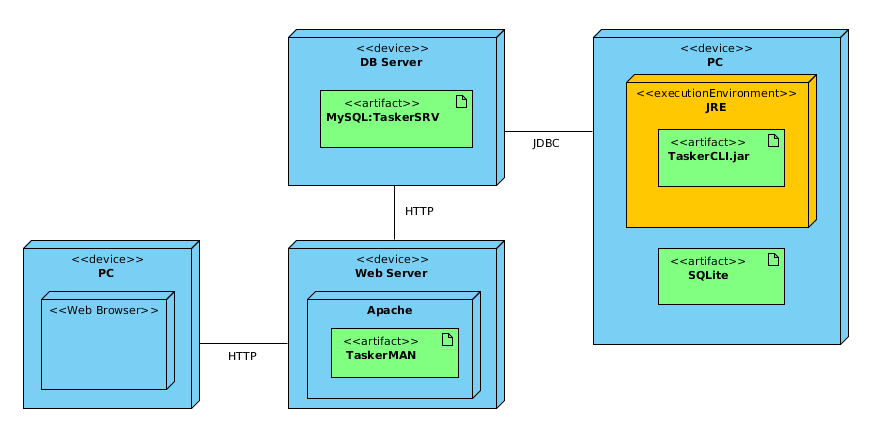
\includegraphics[width=\textwidth]{images/4.1/DeploymentDiagram} \\
The whole system will be composed of the following three components:
\begin{itemize}
	\item TaskerSRV (Database)
	\item TaskerMAN (Web Client)
	\item TaskerCLI (Desktop Client)
\end{itemize} 
TaskerSRV will be deployed onto a database server with a pre-installed MySQL
engine. It will store the critical data of the whole system and make it
accessible to both web and desktop clients through the specified protocols.
TaskerMAN will be deployed as a PHP web application onto an Apache web server
and it will be accessible from the Internet by any client with an installed web 
browser. Finally, TaskerCLI will be a desktop application written in Java, and it
will be deployed as a runnable jar onto a machine running the Java Runtime
Environment. Following the requirements specification\cite{se.qa.rs fr8 local storage}, TaskerCLI will have to
operate both on-line and off-line. Therefore it will have a direct access to 
a local storage provided by the SQLite database.
\subsection{Applications interface}
Unlike the deployment diagram above, the component diagram below depicts the interaction of different modules or components of the proposed system. There are four major components that form the entire system. Only a black box view is shown here. This means that the components are not further decomposed to reveal the inner components. The opposite of this is a white box view which shows not only the major component but also the inner components that form the big picture. 
According to the design specification standard[1], only the simple black box view application interaction is relevant for now. A rundown of the actual interactions is as follows: \\
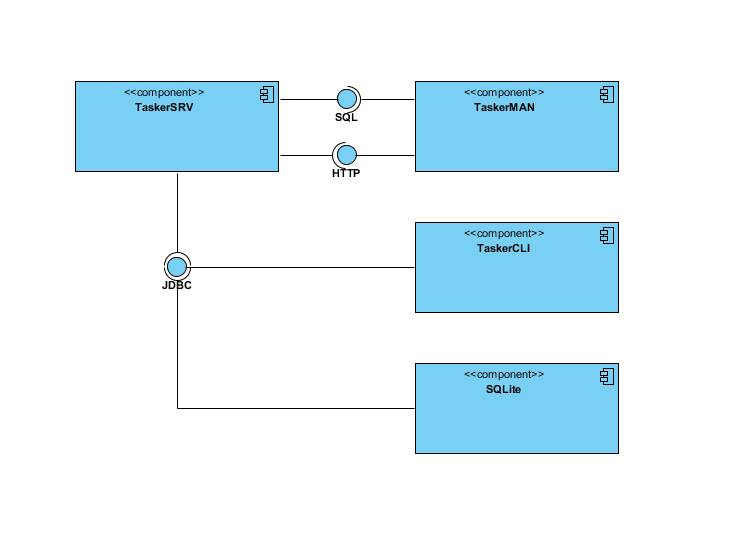
\includegraphics[width=\textwidth]{images/4.2/ApplicationsInterface} 
TaskerSRV - This component, representing the database, consists of one provided interface (solid circle) and two required interfaces (cup shaped). These are:
\begin{itemize}
	\item SQL(provided interface) : Provides an SQL interface, making it possible for the web application, TaskerMAN, to manipulate the database and carry the necessary operations outlined in the requirements[2] such as adding, editing, deleting users or tasks. 
	\item HTTP (required interface): Without the HTTP protocol the database would not be accessed by the TaskerMAN and no operation can take place.
	\item JDBC (required interface): The interface is required so that communication to the SQL can be established and give the required services to the client.
\end{itemize}
TaskerMAN - This component, representing the web application has one required interface (SQL) and one provided interface (HTTP). Without SQL provided by TaskerSRV, TaskerMAN will not be able to do anything. It will remain a useless dummy. Also if it can not provide the HTTP communication interface then it would not be able to access the database. \\
\newline 
TaskerCLI - This component representing the client has one provided interface (JDBC). Since it is using Java to connect to the database, TaskerSRV as well as SQLite will require that the interface JDBC be implemented on the client�or else there will be no database connection. \\
\newline SQLite - This component representing the local database on the client has one required interface (JDBC) which makes it possible for the client to connect to it.
\clearpage
\section{INTERACTION DESIGN}
\subsection{Use-cases}
\subsubsection{TaskerMAN Use-Case}
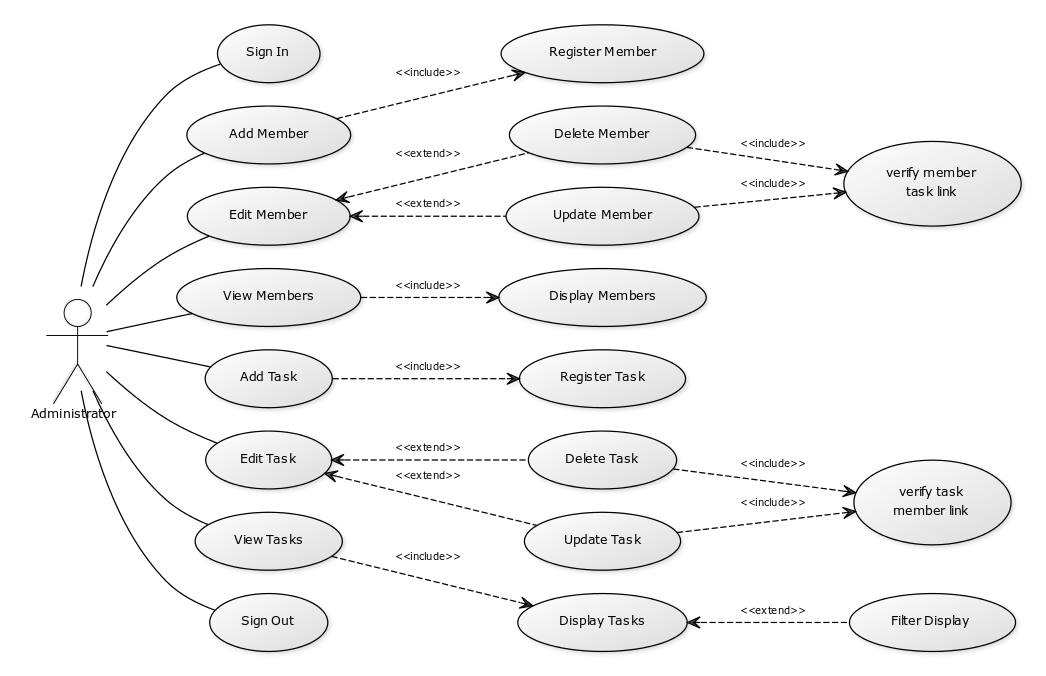
\includegraphics[width=\textwidth]{images/5.1/TaskerMANUseCase}
The TaskerMAN use case diagram above depicts clearly how the web administration application will be able to be used by the administrator.  The necessary functions depicted in the specification requirements[2], are clearly accessible to the administrator after logging into the system. These functionalities are, add task, edit task, view tasks, filter display, add and edit member. The options update member and delete members as well as update task and delete task are labelled as extending.  This is because they are options and an administrator may or may not choose to delete a task or member.  Also they include a verification so that the administrator might be aware, for example, that a member to be deleted or updated might be currently assigned a task or vice versa.  Similarly the filter display is extended since an administrator may choose to filter display results or not.
Example Usage Scenario:
\begin{enumerate}
	\item The administrator logs onto the web application system.
	\item Selects "add member" and registers the members.
	\item Administrator clicks on "view members" to make sure the members are added.
	\item Administrator realises that a member name was misspelled. He or she clicks on "edit member" and selects the option "update member".  Necessary updates are done.
	\item Administrator then clicks on "add task" and a necessary form is displayed where data is entered.
	\item Administrator decides that the task was allocated to the wrong member.  He or she clicks on "edit task".  An appropriate page is loaded where the task can be selected and a reallocation can be carried out.
	\item Administrator decides that one more task is actually not needed.  He or she clicks on "edit task", selects the task and clicks on "delete task".  A prompt is displayed informing that the task is associated with a member.  If the administrator is comfortable to delete, then the action is executed.
	\item Administrator clicks on "view tasks" and all the tasks displayed.  An option is also available for the administrator to filter display results accordingly as specified in the requirements[8].
	\item The administrator has finished using the system and he or she clicks on "log out" and the session ends.
\end{enumerate} 
\subsubsection{TaskerCLI Use-Case}

*insert image here* 

\subsection{User Interface design}
\subsubsection{TaskerMAN Interface Design} 
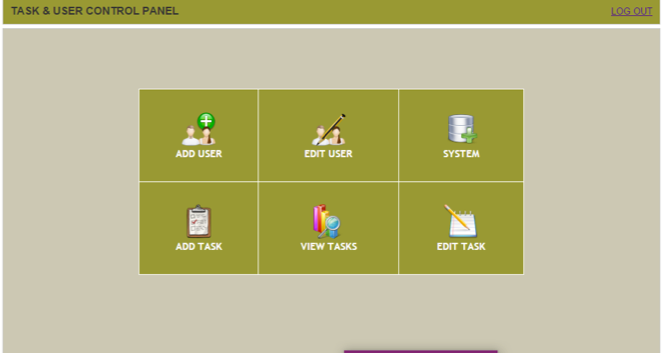
\includegraphics[width=0.75\textwidth, center]{images/5.2/TaskerMANHomePage} \\
This is the home page of the web interface, it is very easy to use and presents you with six options which provides very quick access to all aspects of the Tasker. To begin we will click on the 'Add User' button. This will re-direct us to the 'Add Team Member' page. \\~\\
\newline
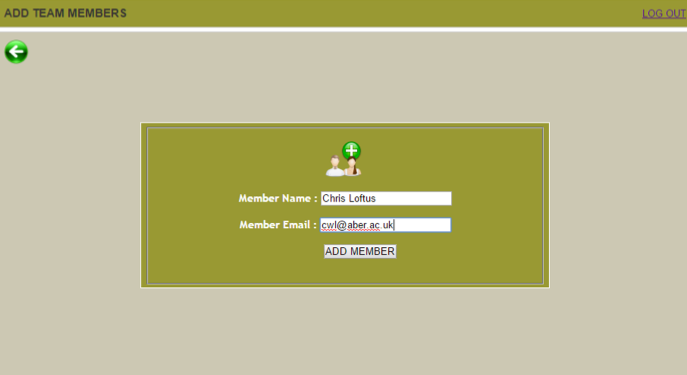
\includegraphics[width=0.75\textwidth, center]{images/5.2/TaskerMANAddUser} \\
Here within the 'Add Team Member' page you will be presented with the form above which then enables you to create a user by presenting their name and e-mail. Upon pressing the 'Add member' button the new member will be added to the database as required \cite{se.qa.rs fr3}. Clicking on the 'backwards arrow' in the top-left corner allows users to return to the home page. In fact the 'backwards arrow' exists within all of the sites internal pages and serves the same function of returning to the home page. \\~\\
\newline
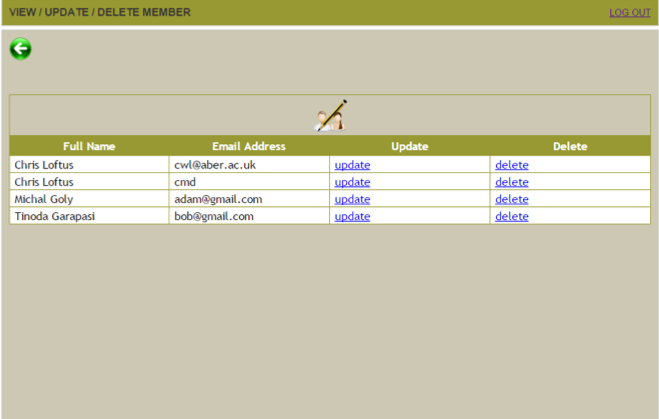
\includegraphics[width=0.75\textwidth, center]{images/5.2/TaskerMANEditUser} \\
To update or delete user data as required \cite{se.qa.rs fr3} click on the 'Edit User' button from the home page and you will be presented with this page, displaying users' names, e-mail addresses and options to update/delete, clicking 'update' re-directs to a page with the same interface as the 'Add Team Member' page where name and e-mail can be updated, clicking 'delete' will prompt the user to verify with a 'confirm'/'cancel' option that they are sure they want to proceed, before re-directing them to a page confirming their deletion and a delete command will be submitted to the database to remove the user from the database. \\~\\
\newline
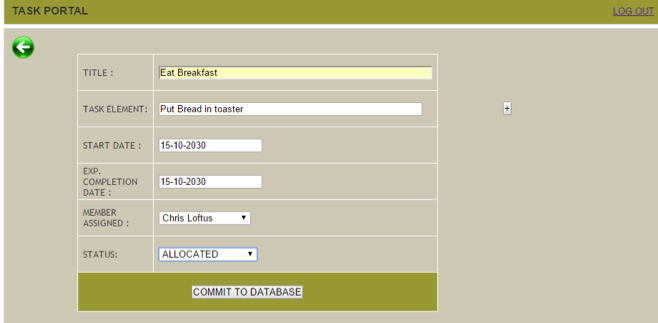
\includegraphics[width=0.75\textwidth, center]{images/5.2/TaskerMANAddTask} \\
Clicking 'Add Task' from the home page will re-direct to the task portal, This is where people can make tasks which will then be submitted to specific users \cite{se.qa.rs fr4}. This task portal layout will also be used when updating tasks. 'Title' and 'Title Description' will be text boxes for user input, 'Start Date' and 'End Completion Date' are currently also text boxes, however to improve validation we may add a drop down calendar at both dates. The 'Member's Assigned' box contains a drop-down list of all the members currently added so it makes it easy to assign or re-assign people to specific tasks \cite{se.qa.rs fr5}. 'Status' is also a drop-down list that can be changed between 'Allocated', 'Abandoned' \cite{se.qa.rs fr6}, 'Completed' and 'Not allocated'. The commit to database button then adds the task to the database and will then sync up with the client, a confirmation screen is then shown to show the user that the task has been successfully added. \\~\\
\newline
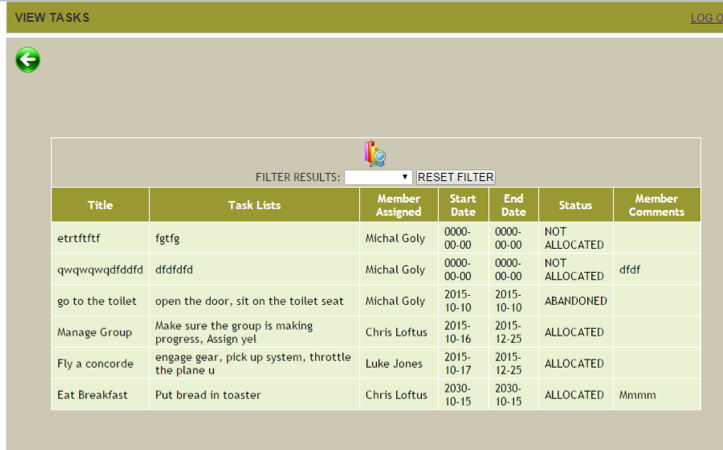
\includegraphics[width=0.75\textwidth, center]{images/5.2/TaskerMANViewTask} \\
To view tasks from the home page the 'view tasks' button must be clicked. This page shows all of the tasks that have been made, you can filter them by using the drop-down box at the top. This list os sorted by expected completion date by default \cite{se.qa.rs fr7}.


\subsubsection{TaskerCLI Interface Design} 
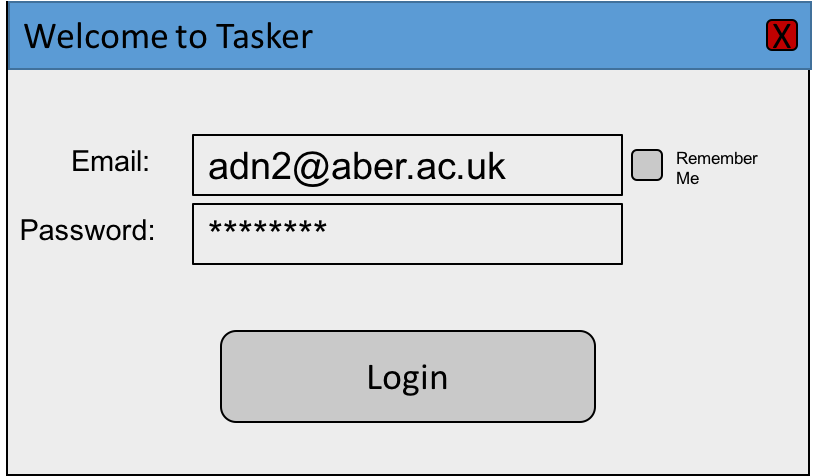
\includegraphics[width=0.5\textwidth, center]{images/5.2/TaskerCLILogin} \\
The login screen, the first screen to appear when the client loads. TaskerCLI does not synchronise with the database until the user has logged in as specified in Requirements Specifications.\cite{se.qa.rs fr8 user id} \\~\\
\newline
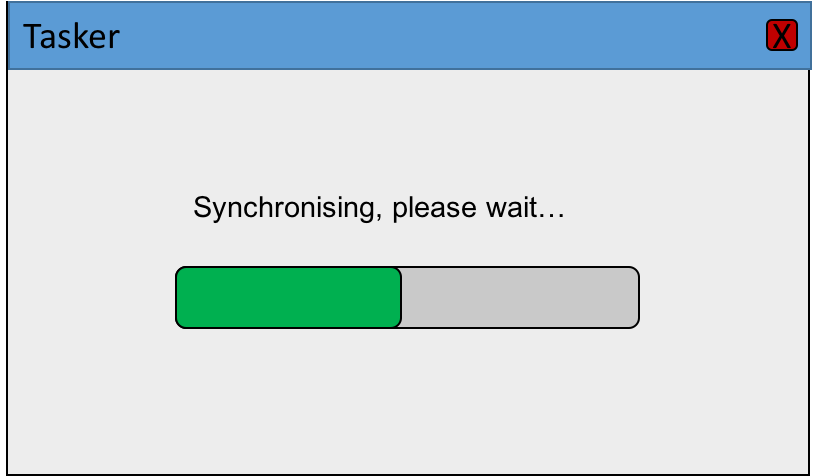
\includegraphics[width=0.5\textwidth, center]{images/5.2/TaskerCLILoading} \\
The synchronisation screen occurs between the login and main client page. As per the requirements specifications \cite{se.qa.rs fr11} this screen will also occur before and after local editing if network access is available, as well as occurring every 5 minutes by default should no local editing take place. This will display the relevant information from the database as it's downloading the data. Ideally this will be a fast enough task that this screen should be seen for as little time as possible. \\~\\
\newline
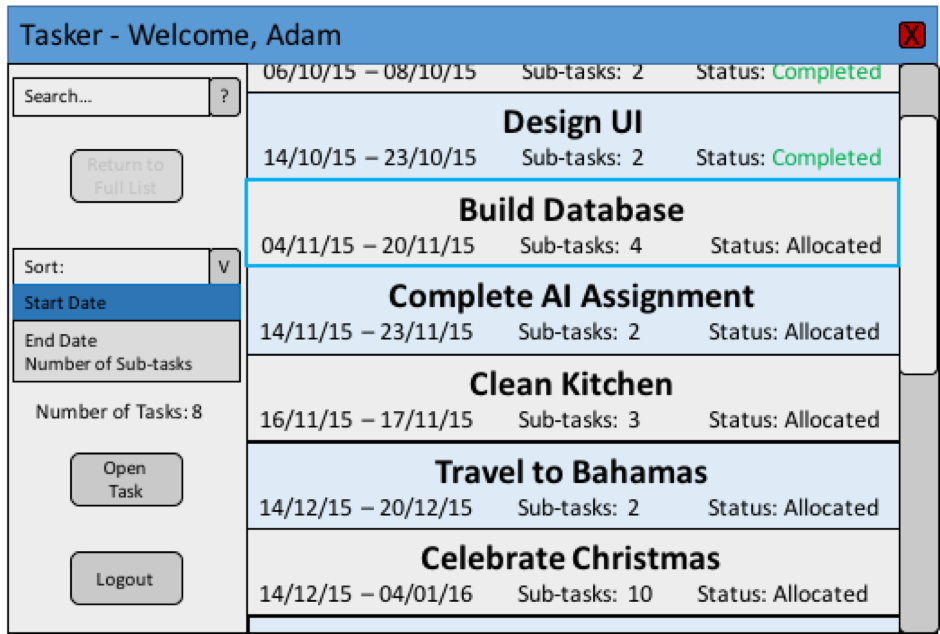
\includegraphics[width=0.75\textwidth, center]{images/5.2/TaskerCLIMainScreen} \\
The 'Main Screen' of TaskerCLI. It shows a list of tasks assigned to the person who signed in, as well as options for sorting and searching through the list. Clicking on the 'Log Out' button will re-direct the user back to the login authentication screen. Double clicking a task's panel, or selecting a task and clicking the 'open task' button shows more detail about the task \cite{se.qa.rs fr10}, as well as the editable parts, such as the completed/allocated attribute and the sub-task list comments. In this example we'll double-click on the "Build Database" task. \\~\\
\newline
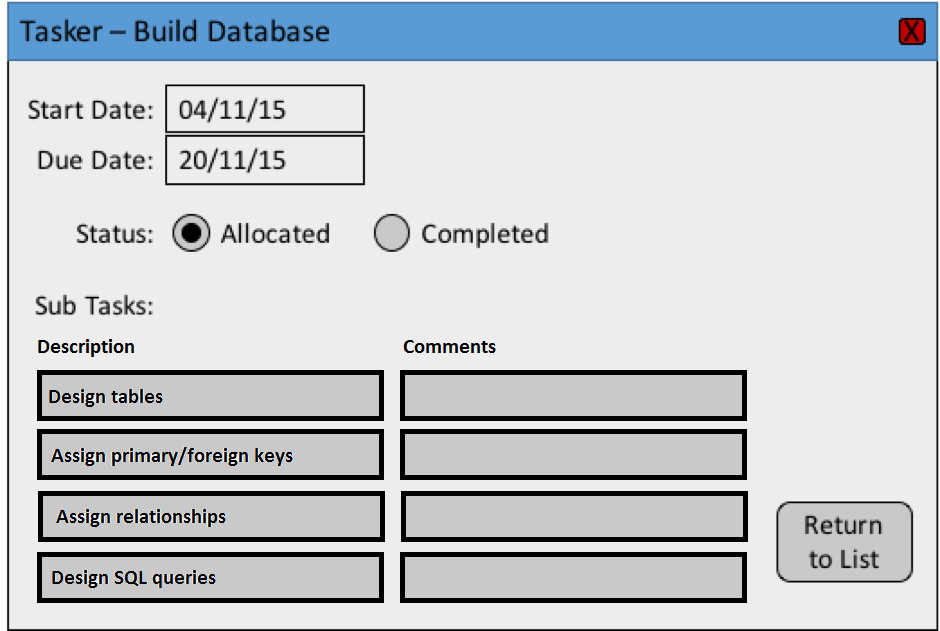
\includegraphics[width=0.75\textwidth, center]{images/5.2/TaskerCLITaskInfo} \\
This screen shows more details about the "Build Database". It displays all the task's information and allows the user to edit task step comments and change task's status \cite{se.qa.rs fr10}. \\~\\
\newline
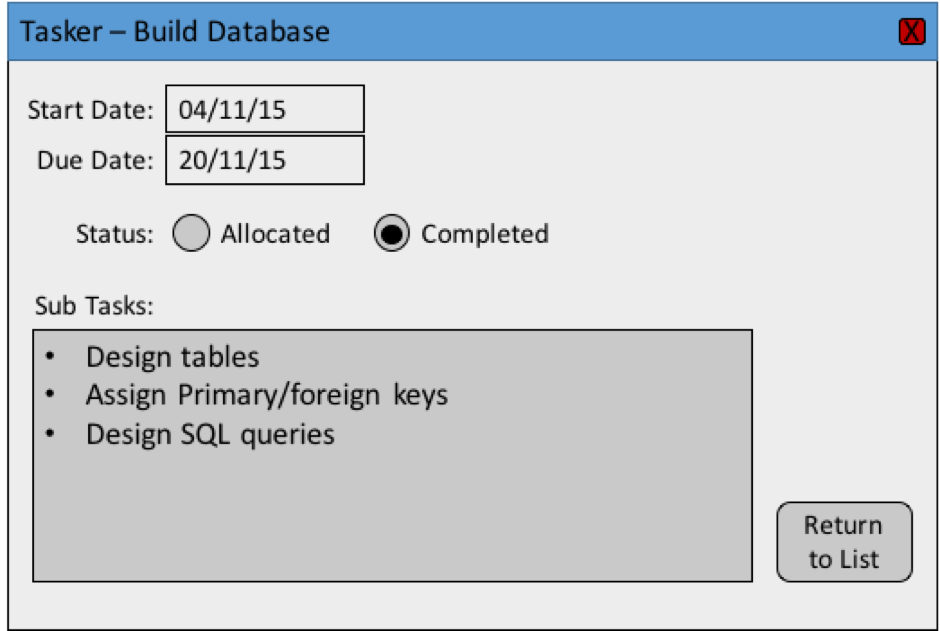
\includegraphics[width=0.75\textwidth, center]{images/5.2/TaskerCLITaskUpdated} \\
In this image we've changed the status to 'Completed'. We can press the 'Return to List' button to return to the 'Main Screen'. Doing so will prompt the synchronisation screen to appear and an attempt will be made to connect to the network and update the information on the remote MySQL database. If unsuccessful the user will still be re-directed back to the 'Main Screen', however the client will be now operating locally using the local SQLite database until a connection with the MySQL can be re-established.\\~\\
\newline
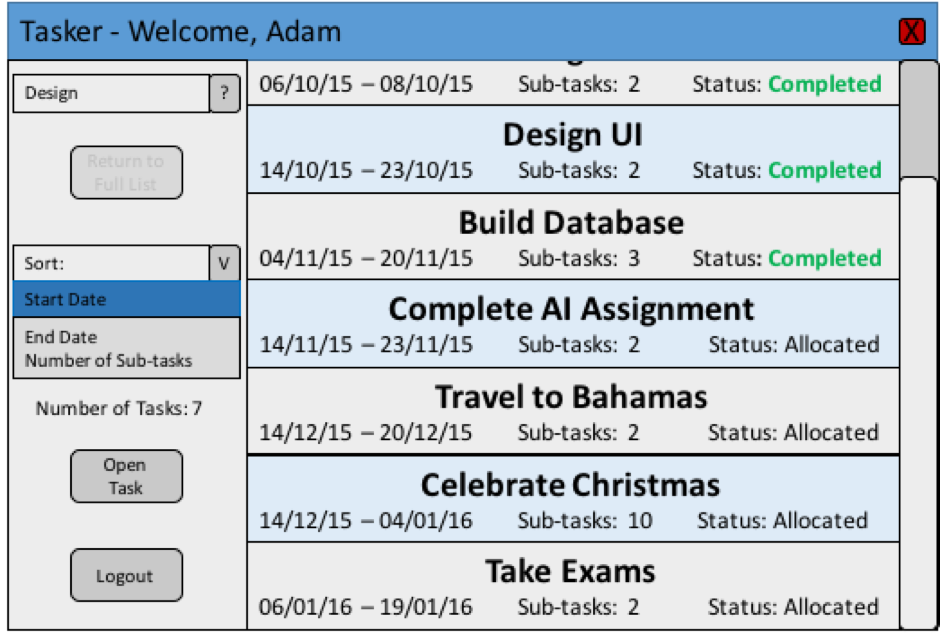
\includegraphics[width=0.75\textwidth, center]{images/5.2/TaskerCLIMainScreenUpdated} \\
Note the changes made are now reflected in this list. Also note that the task named 'Clean Kitchen' has disappeared. This is something that could happen if said task were marked 'Abandoned' via TaskerMAN while the user was editing a task within TaskerCLI, provided there is a network connection. \\~\\
\newline
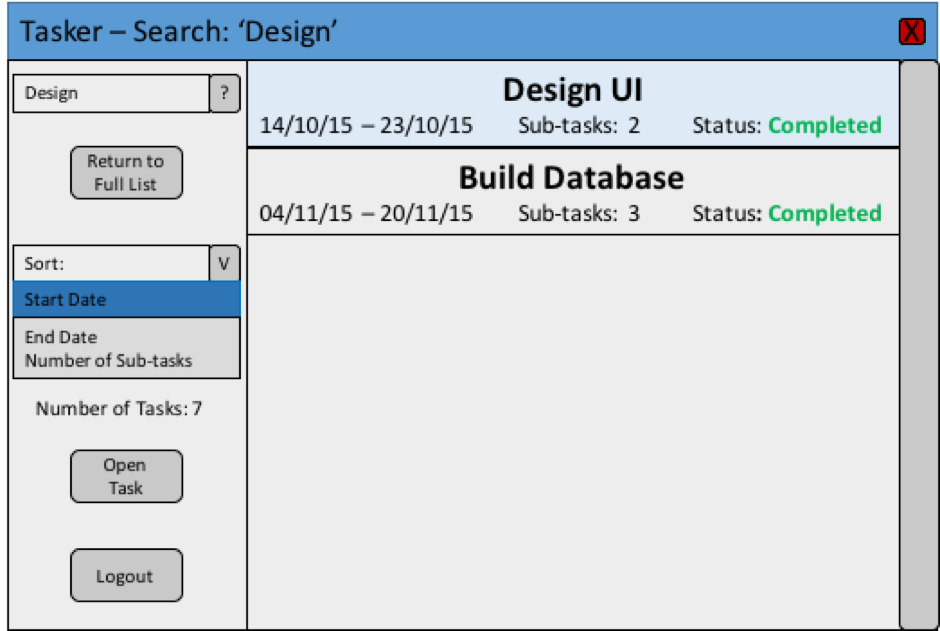
\includegraphics[width=0.75\textwidth, center]{images/5.2/TaskerCLIMainScreenSearch} \\
Searching using the text box searches for the string provided in the task's name, and/or it's sub-tasks. Also note that the 'return to full list' button is only selectable if there is currently a search parameter in the search box.\\~\\
\newline
There is a large focus on designing the interfaces of both TaskerCLI and TaskerMAN to be intuitive to regular computer users \cite{se.qa.rs ir1}.
\clearpage
\addcontentsline{toc}{section}{REFERENCES}
\begin{thebibliography}{12}
\bibitem{se.qa.ds} \emph{Software Engineering Group Projects}
Design Specification Standards.
C. J. Price, N.W.Hardy and B.P.Tiddeman, SE.QA.05A. 1.8 Release.
\bibitem{se.qa.rs} \emph{Software Engineering Group Projects}
Requirements Specifications.
N. W. Hardy, SE.QA.RS. 1.1 Release.
\bibitem{se.qa.rs fr8 local storage} \emph{Software Engineering Group Projects}
Requirements Specifications.
N. W. Hardy, SE.QA.RS, FR8 \emph{Local Storage of Tasks}. 1.1 Release.
\bibitem{se.qa.rs fr3} \emph{Software Engineering Group Projects}
Requirements Specifications.
N. W. Hardy, SE.QA.RS, FR3. 1.1 Release.
\bibitem{se.qa.rs fr4} \emph{Software Engineering Group Projects}
Requirements Specifications.
N. W. Hardy, SE.QA.RS, FR4. 1.1 Release.
\bibitem{se.qa.rs fr5} \emph{Software Engineering Group Projects}
Requirements Specifications.
N. W. Hardy, SE.QA.RS, FR5. 1.1 Release.
\bibitem{se.qa.rs fr6} \emph{Software Engineering Group Projects}
Requirements Specifications.
N. W. Hardy, SE.QA.RS, FR6. 1.1 Release.
\bibitem{se.qa.rs fr7} \emph{Software Engineering Group Projects}
Requirements Specifications.
N. W. Hardy, SE.QA.RS, FR7. 1.1 Release.
\bibitem{se.qa.rs fr8 user id} \emph{Software Engineering Group Projects}
Requirements Specifications.
N. W. Hardy, SE.QA.RS, FR8 \emph{User Identification}. 1.1 Release.
\bibitem{se.qa.rs fr11} \emph{Software Engineering Group Projects}
Requirements Specifications.
N. W. Hardy, SE.QA.RS, FR11. 1.1 Release.
\bibitem{se.qa.rs fr10} \emph{Software Engineering Group Projects}
Requirements Specifications.
N. W. Hardy, SE.QA.RS, FR10. 1.1 Release.
\bibitem{se.qa.rs ir1} \emph{Software Engineering Group Projects}
Requirements Specifications.
N. W. Hardy, SE.QA.RS, IR1. 1.1 Release.
\end{thebibliography}
\clearpage
\addcontentsline{toc}{section}{DOCUMENT HISTORY}
\section*{DOCUMENT HISTORY}
\begin{tabular}{|l | l | l | p{8cm} |l | }
\hline
Version & CCF No. & Date & Changes made to Document & Changed by \\
\hline
1.0 & N/A & 2015-10-27 & Initial creation for review & L. Jones \\
\hline
1.1 & N/A & 2015-10-28 & Updated the TaskerCLI user interface section & M. Goly \\
\hline
1.2 & N/A & 2015-10-28 & Created sub-subsections for  Use-cases and User-inerface design subsections, updated TaskerMAN Task Portal image and information, minor grammatical revision document-wide & L. Jones \\
\hline
\end{tabular}
\label{thelastpage}
\end{document}
\end{verbatim}
\label{fig:footer}
\end{figure}
\label{thelastpage}
\end{document}
